\section{Meta-heuristic optimisation of the charging station placement}
\label{sec:opt}



In the previous section, we saw how the \textit{Num Parking} placement heuristic works better than the other two.
%With more than 5\% of zones, the system sustains itself, both with the \textit{Needed} and the \textit{Hybrid} return policy. 
Weighting also charges and rerouting, the \textit{Hybrid} policy shows better performances than \textit{Needed}. For this reason, in this section, we focus on the \textit{Hybrid} return policy with charging stations covering less than 15\% of the zones. We further optimise this scenario by running the meta-heuristic placement algorithms, and comparing the results with the \textit{Num Parking} placement. 
Optimisation with \textit{Needed} return policies are briefly discussed in \ref{sec:needed}, where very similar results are obtained.  

%Despite the good performances of the heuristic approach from Fig. \ref{fig:global_weighted_distance} the customer has to walk a lot when rerouted. For this reason in this section, we exploit two optimization algorithms to improve previous results. 
%We exploit the two optimization algorithms described in Sec. \ref{sec:optmizers}.
The hill-climbing local search, here abbreviated in \textit{Local Search}, uses \textit{Num Parking} placement as initial solution. The \textit{Genetic} algorithm creates a totally new solution without exploiting any previous knowledge. 
Recall that both algorithms are designed to find the best charging stations placement that guarantee 0 infeasibile trips, and to minimise the overall distance the customer has to walk to reach the final destination.


\begin{figure}[th]
    \centering     %%% not \center
    \subfloat[][Percentage of infeasible trips.  Y-Axis is logarithmic.]
    {
      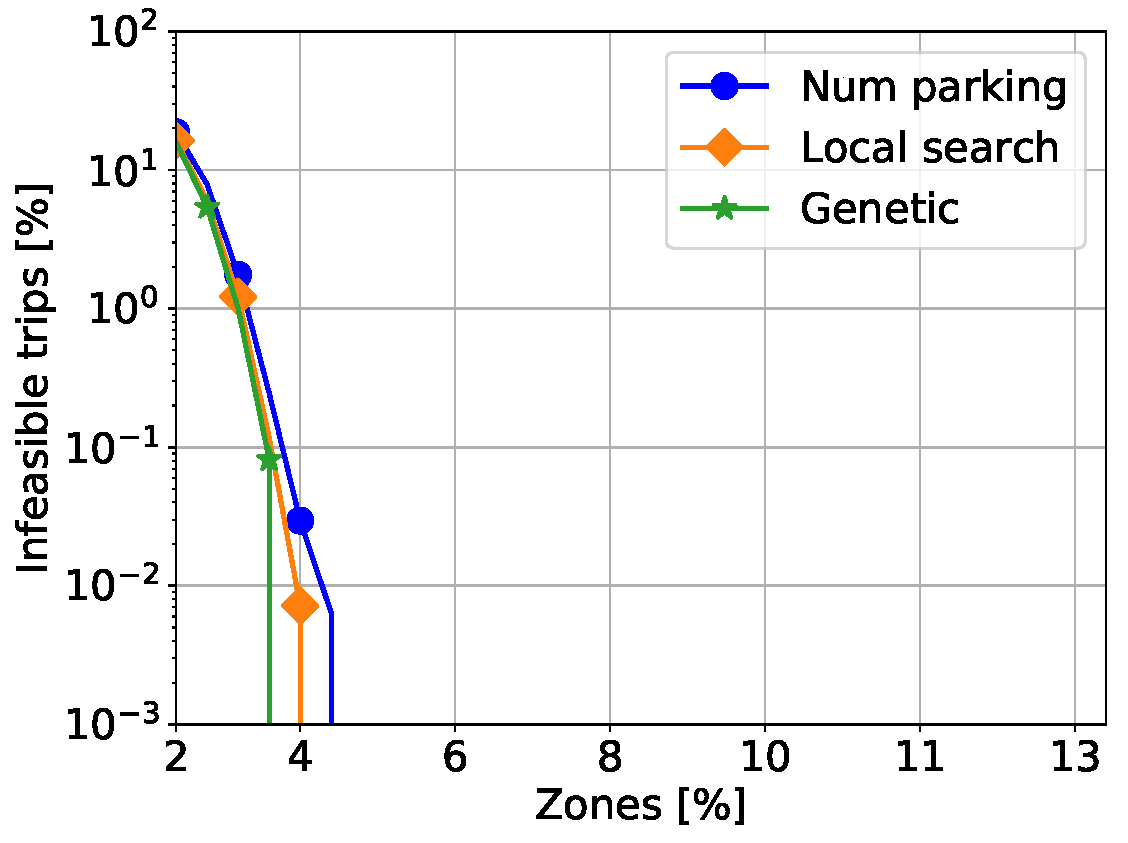
\includegraphics[width=0.45\textwidth]{figures/Hybrid_Deaths.pdf}
        \label{fig:optimized_deaths}
    }
    \subfloat[][Average walked distance.]
    {
        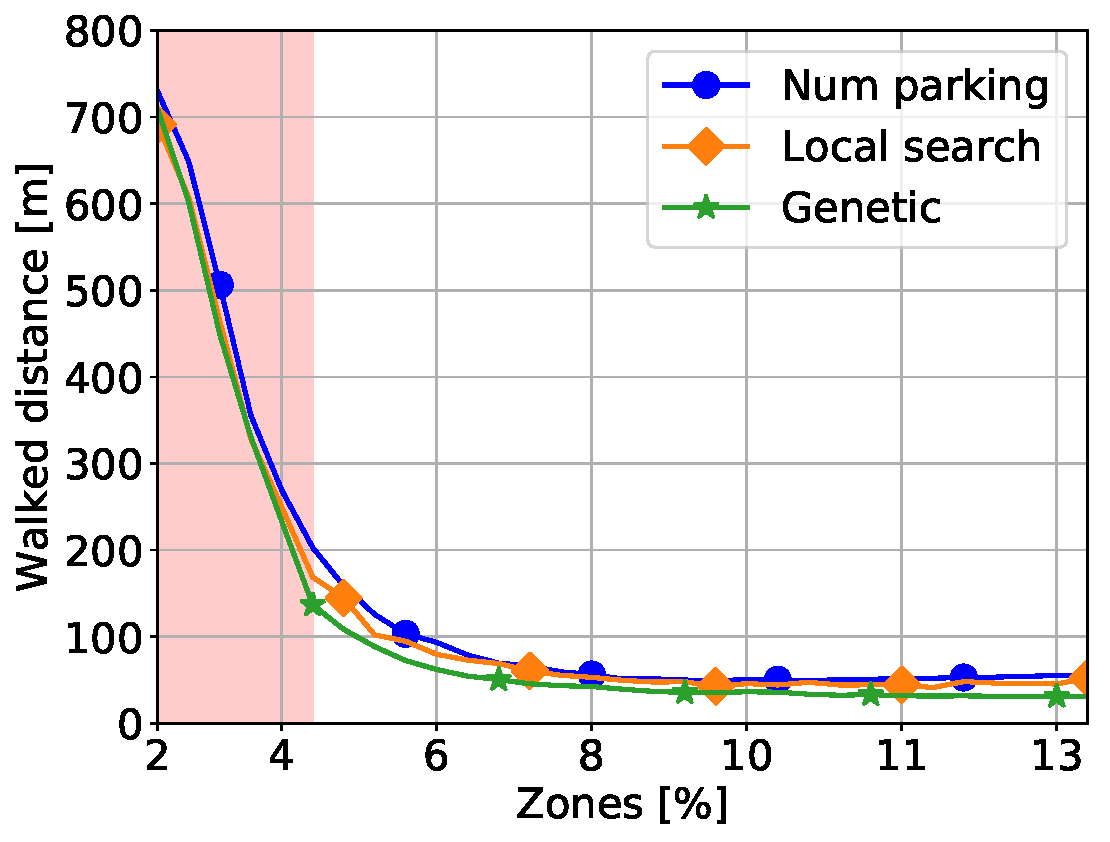
\includegraphics[width=0.45\textwidth]{figures/Hybrid_TravelWithPenlaty.pdf}
        \label{fig:optimized_penaly}
    }    
    \label{fig:optimized_metrics}
    \caption{Objective metrics to minimise in the optimisation - with \textit{Hybrid} return policy.}
\end{figure}


\begin{figure}[th]
    \centering     %%% not \center
    
    \subfloat[][Percentage of trips ending with a charge.]
    {
        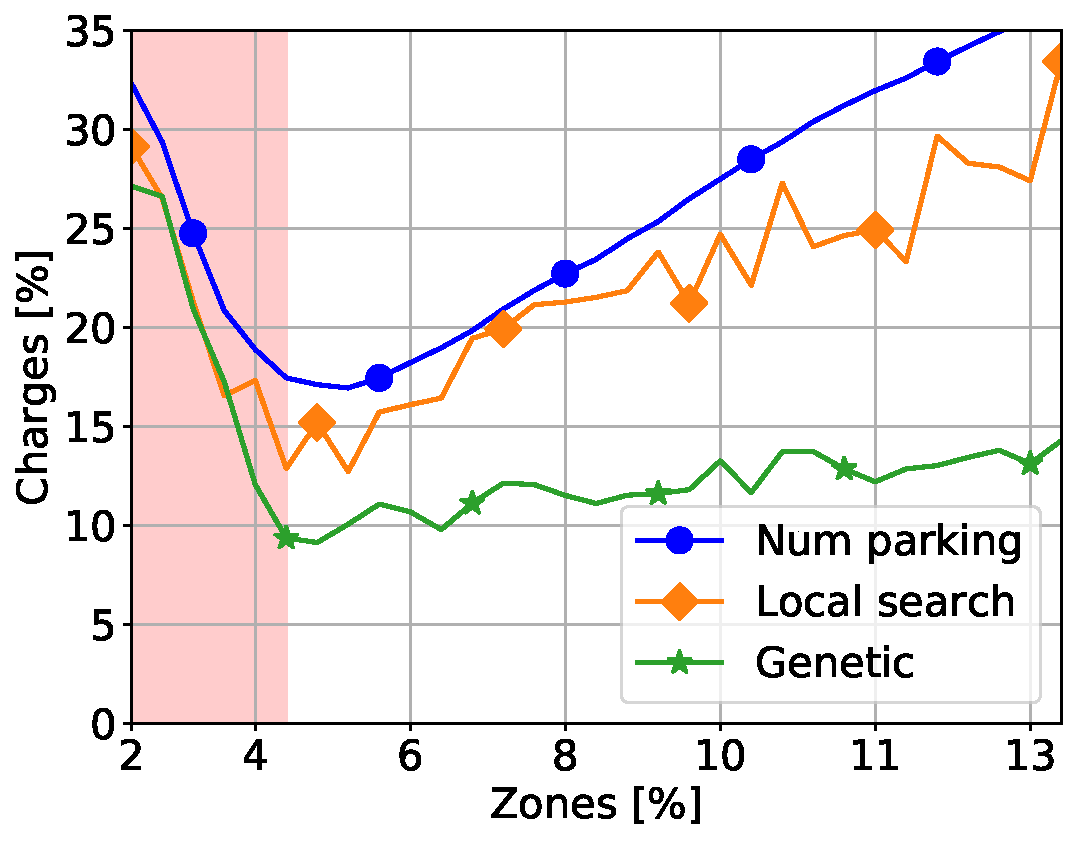
\includegraphics[width=0.45\textwidth]{figures/Hybrid_AmountRechargePerc.pdf}
        \label{fig:recharge}
    }
    \subfloat[][Average state of charge.]
    {
        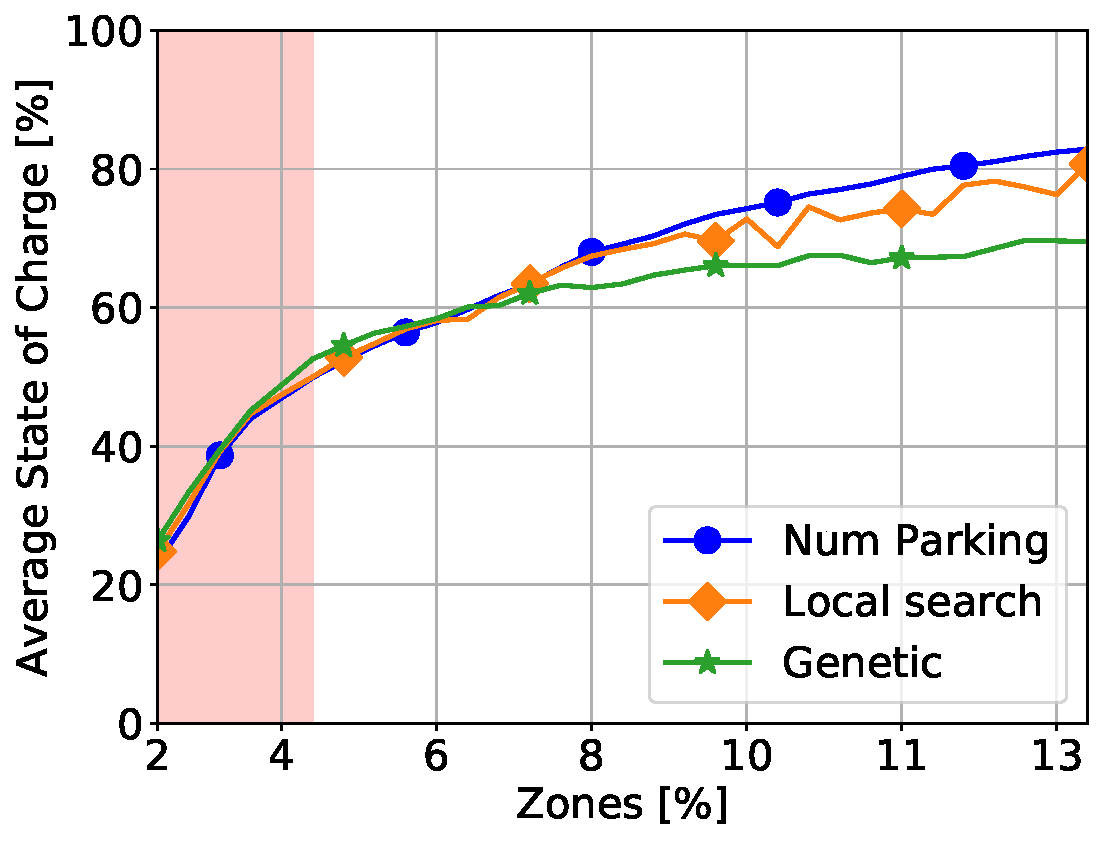
\includegraphics[width=0.45\textwidth]{figures/AvgSOC_comparison.pdf}
        \label{fig:asoc}
    }     
    \subfloat[][Rerouted trips percentage.]
    {
        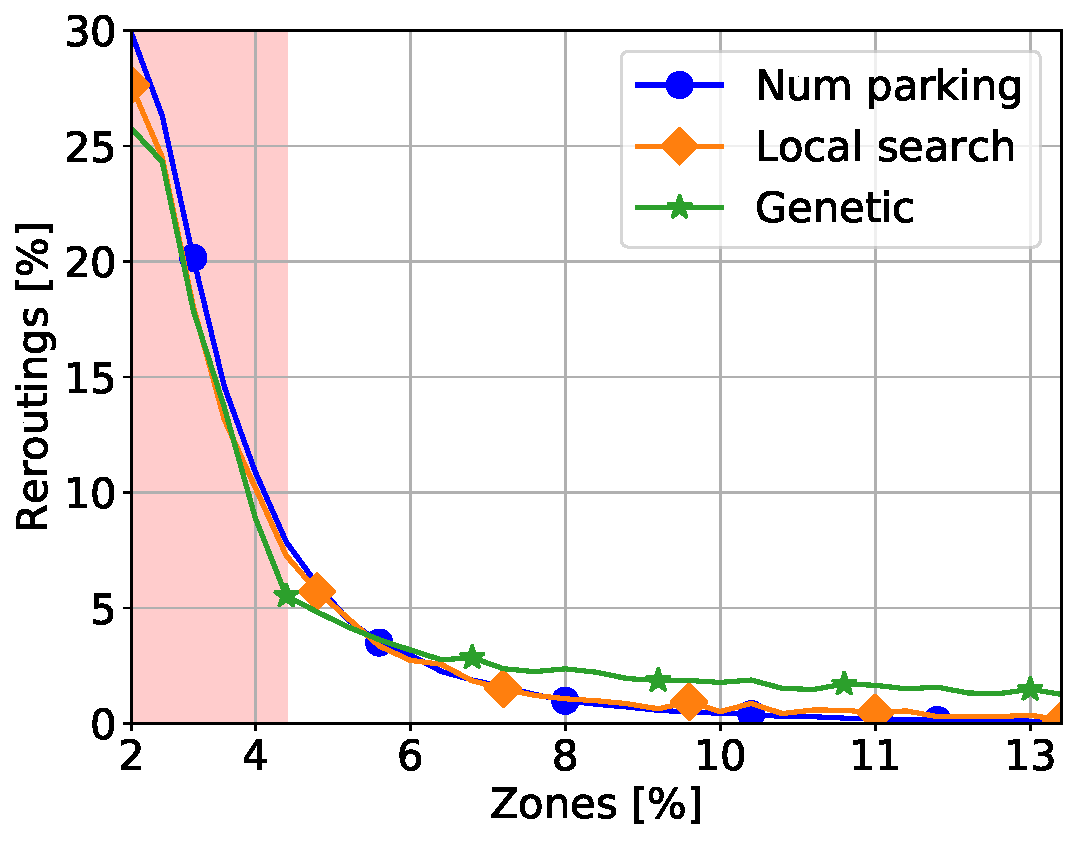
\includegraphics[width=0.45\textwidth]{figures/Hybrid_ReroutePerc.pdf}
        \label{fig:reroute}
    } 
% \subfigure[Walked distance, averaged over all trips \lv{Cambiare label asse y da Glob. w.w.d a Walked distance (vedere sezione 4.2. e 5.2 per maggiori dettagli)}]
%     {
%         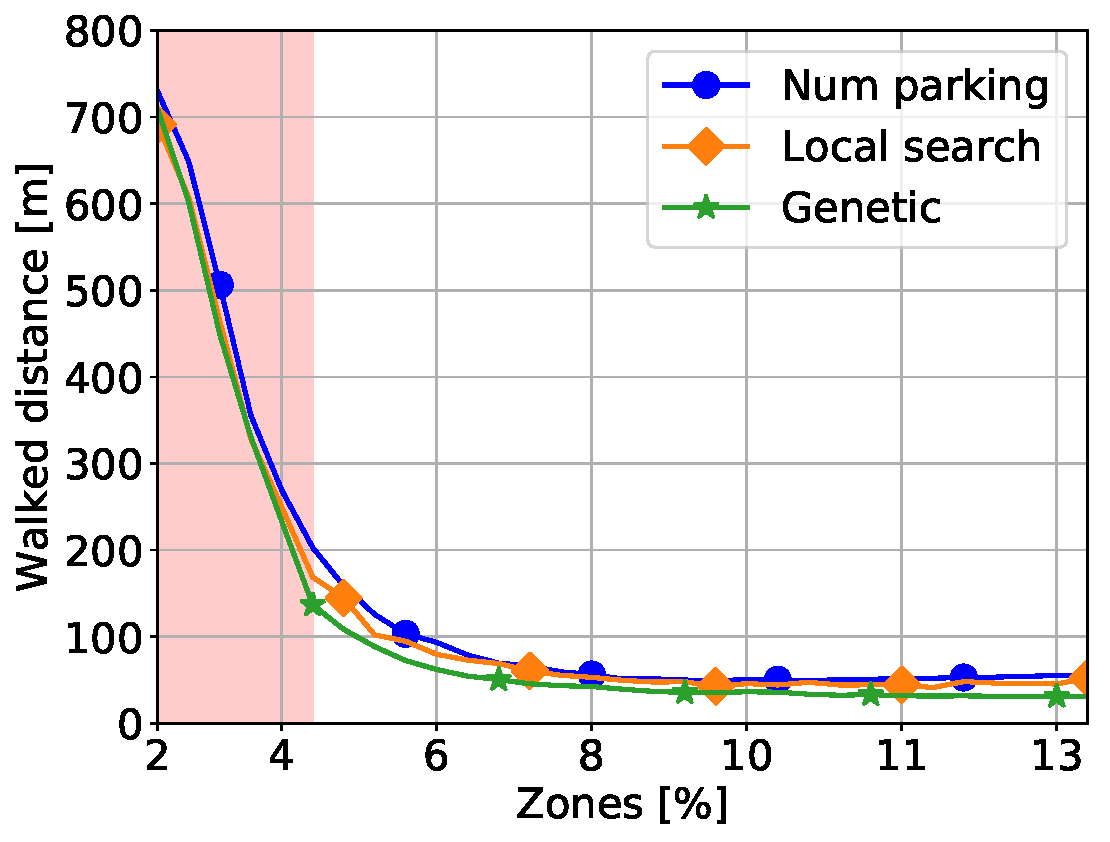
\includegraphics[width=0.3\textwidth]{figures/Hybrid_TravelWithPenlaty.pdf}
%         \label{fig:wwd}
%     }
    \subfloat[][Walked distance when rerouted.]
    {
        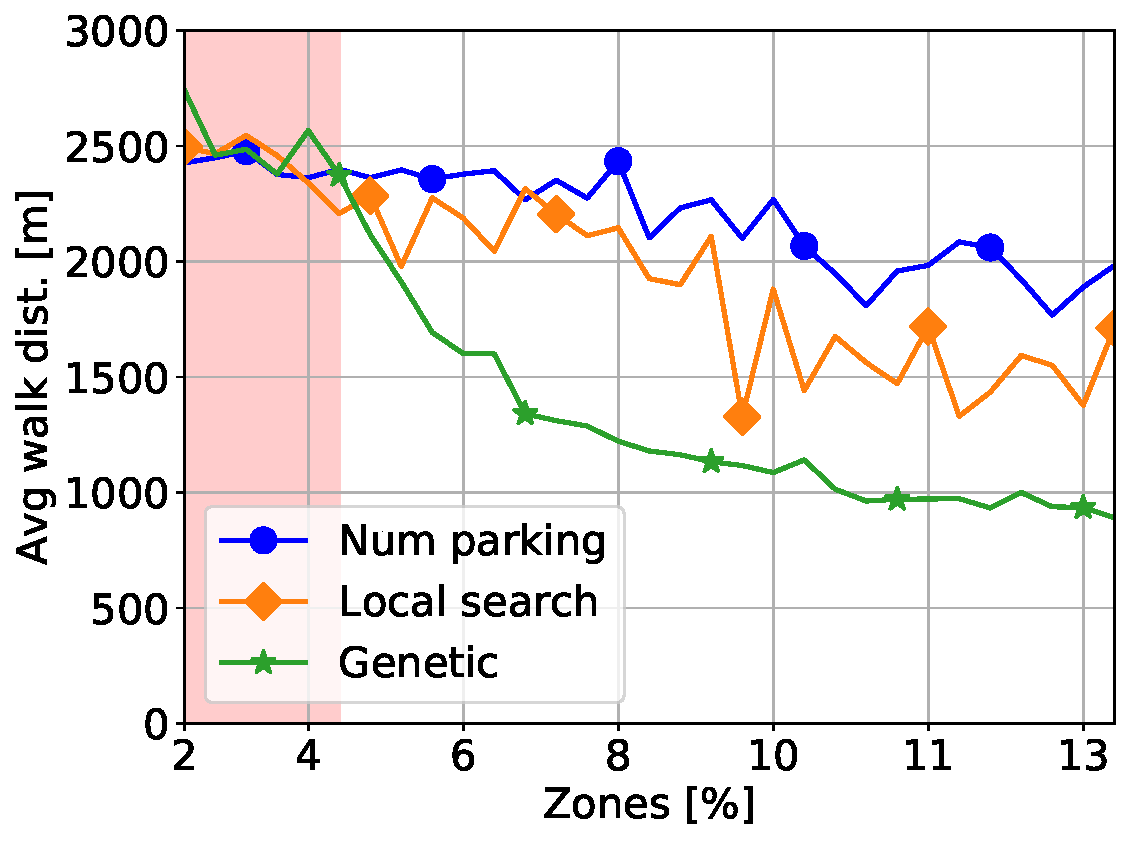
\includegraphics[width=0.45\textwidth]{figures/Hybrid_AvgWalkedDistance.pdf}
        \label{fig:awd}
    }
    \caption{\textit{Genetic} and \textit{Local Search} optimisation results for metrics of interests (\textit{Hybrid} return policy adopted). }
    \label{fig:hybrid_optimization}
\end{figure}


Fig.~\ref{fig:optimized_metrics} reports the two target metrics, for all the optimised configurations.
Firstly, in Fig.~\ref{fig:optimized_deaths} we compare the infeasible trip percentage. \textit{Num Parking} solution (blue line) has already good performance, reaching 0 with 4.2\% of the equipped zones. 
The \textit{Local Search} (orange line) and the \textit{Genetic} (green line) algorithms are able to further reduce the minimum percentage of zone to equip to guarantee no infeasible trips: 3.8\% by the \textit{Local Search}, and to 3.5\% with the \textit{Genetic} algorithm, $Z=10$ and $Z=9$ zones respectively.
%This improvements highlight that (i) \textit{Num Parking} is not the best overall placement, and (ii) local search reaches only a local optimum. 
%This improvements highlight that in the one hand, the \textit{Num Parking} solution represents a very good starting points to place charging stations. In the other hand, they prove that \textit{Num Parking} is not the best placement algorithm overall, since by using a solution not derived from it, we can achieve better performance.  
%The second objective of our optimizer is to improve the customer discomfort in terms of overall distance the customers have to walk to reach the final destination (

Fig.~\ref{fig:optimized_penaly} reports the walked distance. Focusing in the feasible region, the \textit{Genetic} algorithm confirms the best performance, reducing the distance from more than 200\,m to 136\,m when 4.2\% of the zones are equipped with charging stations, and reaching just 30\,m at 13\%. 




In Fig.~\ref{fig:hybrid_optimization} we further study the new solutions on other metrics.
Fig. \ref{fig:recharge} reports the percentage of trips ending in a charging station. The more charges are performed, the more time the customer has to spend time plugging/unplugging the car. By minimising the walked distance, we also reduce this metric, since a trip ending with a charge corresponds to 150\,m of penalty.
Here, the \textit{Local Search} follows the same trend as the \textit{Num parking} with a strong rise. The \textit{Genetic} algorithm shows much better results, from 9\% to 14\% of trips ending with a charge -- half of those found with other solutions. 
This improvement highlights the better placement of the charging stations.
Focus now on Fig. \ref{fig:asoc}, which reports the average state of charge of the car battery. 
No major difference are observed here, with all curves almost overlapping up to 7\% of the zones.

In a nutshell, the solution found by the \textit{Genetic} algorithm lets customers charge much less frequently, while keeping the average state of charge very similar. 
%Despite that in \textit{Genetic} algorithm we plug the car at most 14\% of the time, the average state of charge rise, reaching up to 70\% with 13\% of the zone.

%An other important metric to be evaluated is the percentage of rerouted trips, as the customer may be discouraged by frequent rereoutes. 
Consider next Fig. \ref{fig:reroute}, which details the percentage of reroutes. We can see how the trend is the opposite with respect to the previous ones. Here, the \textit{Genetic} optimised solution show a little higher rerouting percentage than the \textit{Num parking}. 
%Since the \textit{Local Search} and the \textit{Max parking} have similar placement, this percentage does not show particular differences with the two curves almost overlapped. Instead, 
In particular, the \textit{Genetic} algorithm 
%shows a stable reroute percentage with more than 8\% of zones, 
reaches 1.3\% of reroutes, while \textit{Num parking} decreases down to 0.2\% of reroutes. Indeed, the \textit{Genetic} algorithm places charging stations not only where most rentals ends, but also so to decrease the customers' average walked distance, i.e., in those places where likely cars are not so frequently parked but that can be quickly reached in case of rerouting.
To understand the importance of this difference, in Fig.~\ref{fig:awd} we evaluate the walking distance a customer has to walk because she suffered a reroute.  
%As previously shown in Fig. \ref{fig:optimized_penaly}, the optimized algorithms show that, overall, the customer has to walk less than the \textit{Num parking} solution. In particular, Fig. \ref{fig:awd} shows that 
The \textit{Genetic} algorithm is able to push the walked distance below 1\,km, while the \textit{Local Search} generates marginal improvements.
In a nutshell, despite customers are rerouted more frequently, on average, they walk for a shorter, and  more bearable, distance.

% %3.4. usage of poles
% \lv{add plots or even just  sentence about the usage of poles? Usage of pools to show how genetic is better. Asse x numero di zone, asse y Occupazione \% delle paline, per i 3 placement}

In conclusion, a smart placement of the charging stations is better under different perspectives.  The \textit{Genetic} solution, tailored on the data of the usage behaviour, allows us to improve both the system performance, and customers' discomfort, in particular by greatly reducing the number of times they have to charge, and the distance they have to walk.


\subsection{Charging station placement visualisation}

\begin{figure}[h!]
    \centering     %%% not \center
    \subfloat[][Number of Parkings.]
    {
        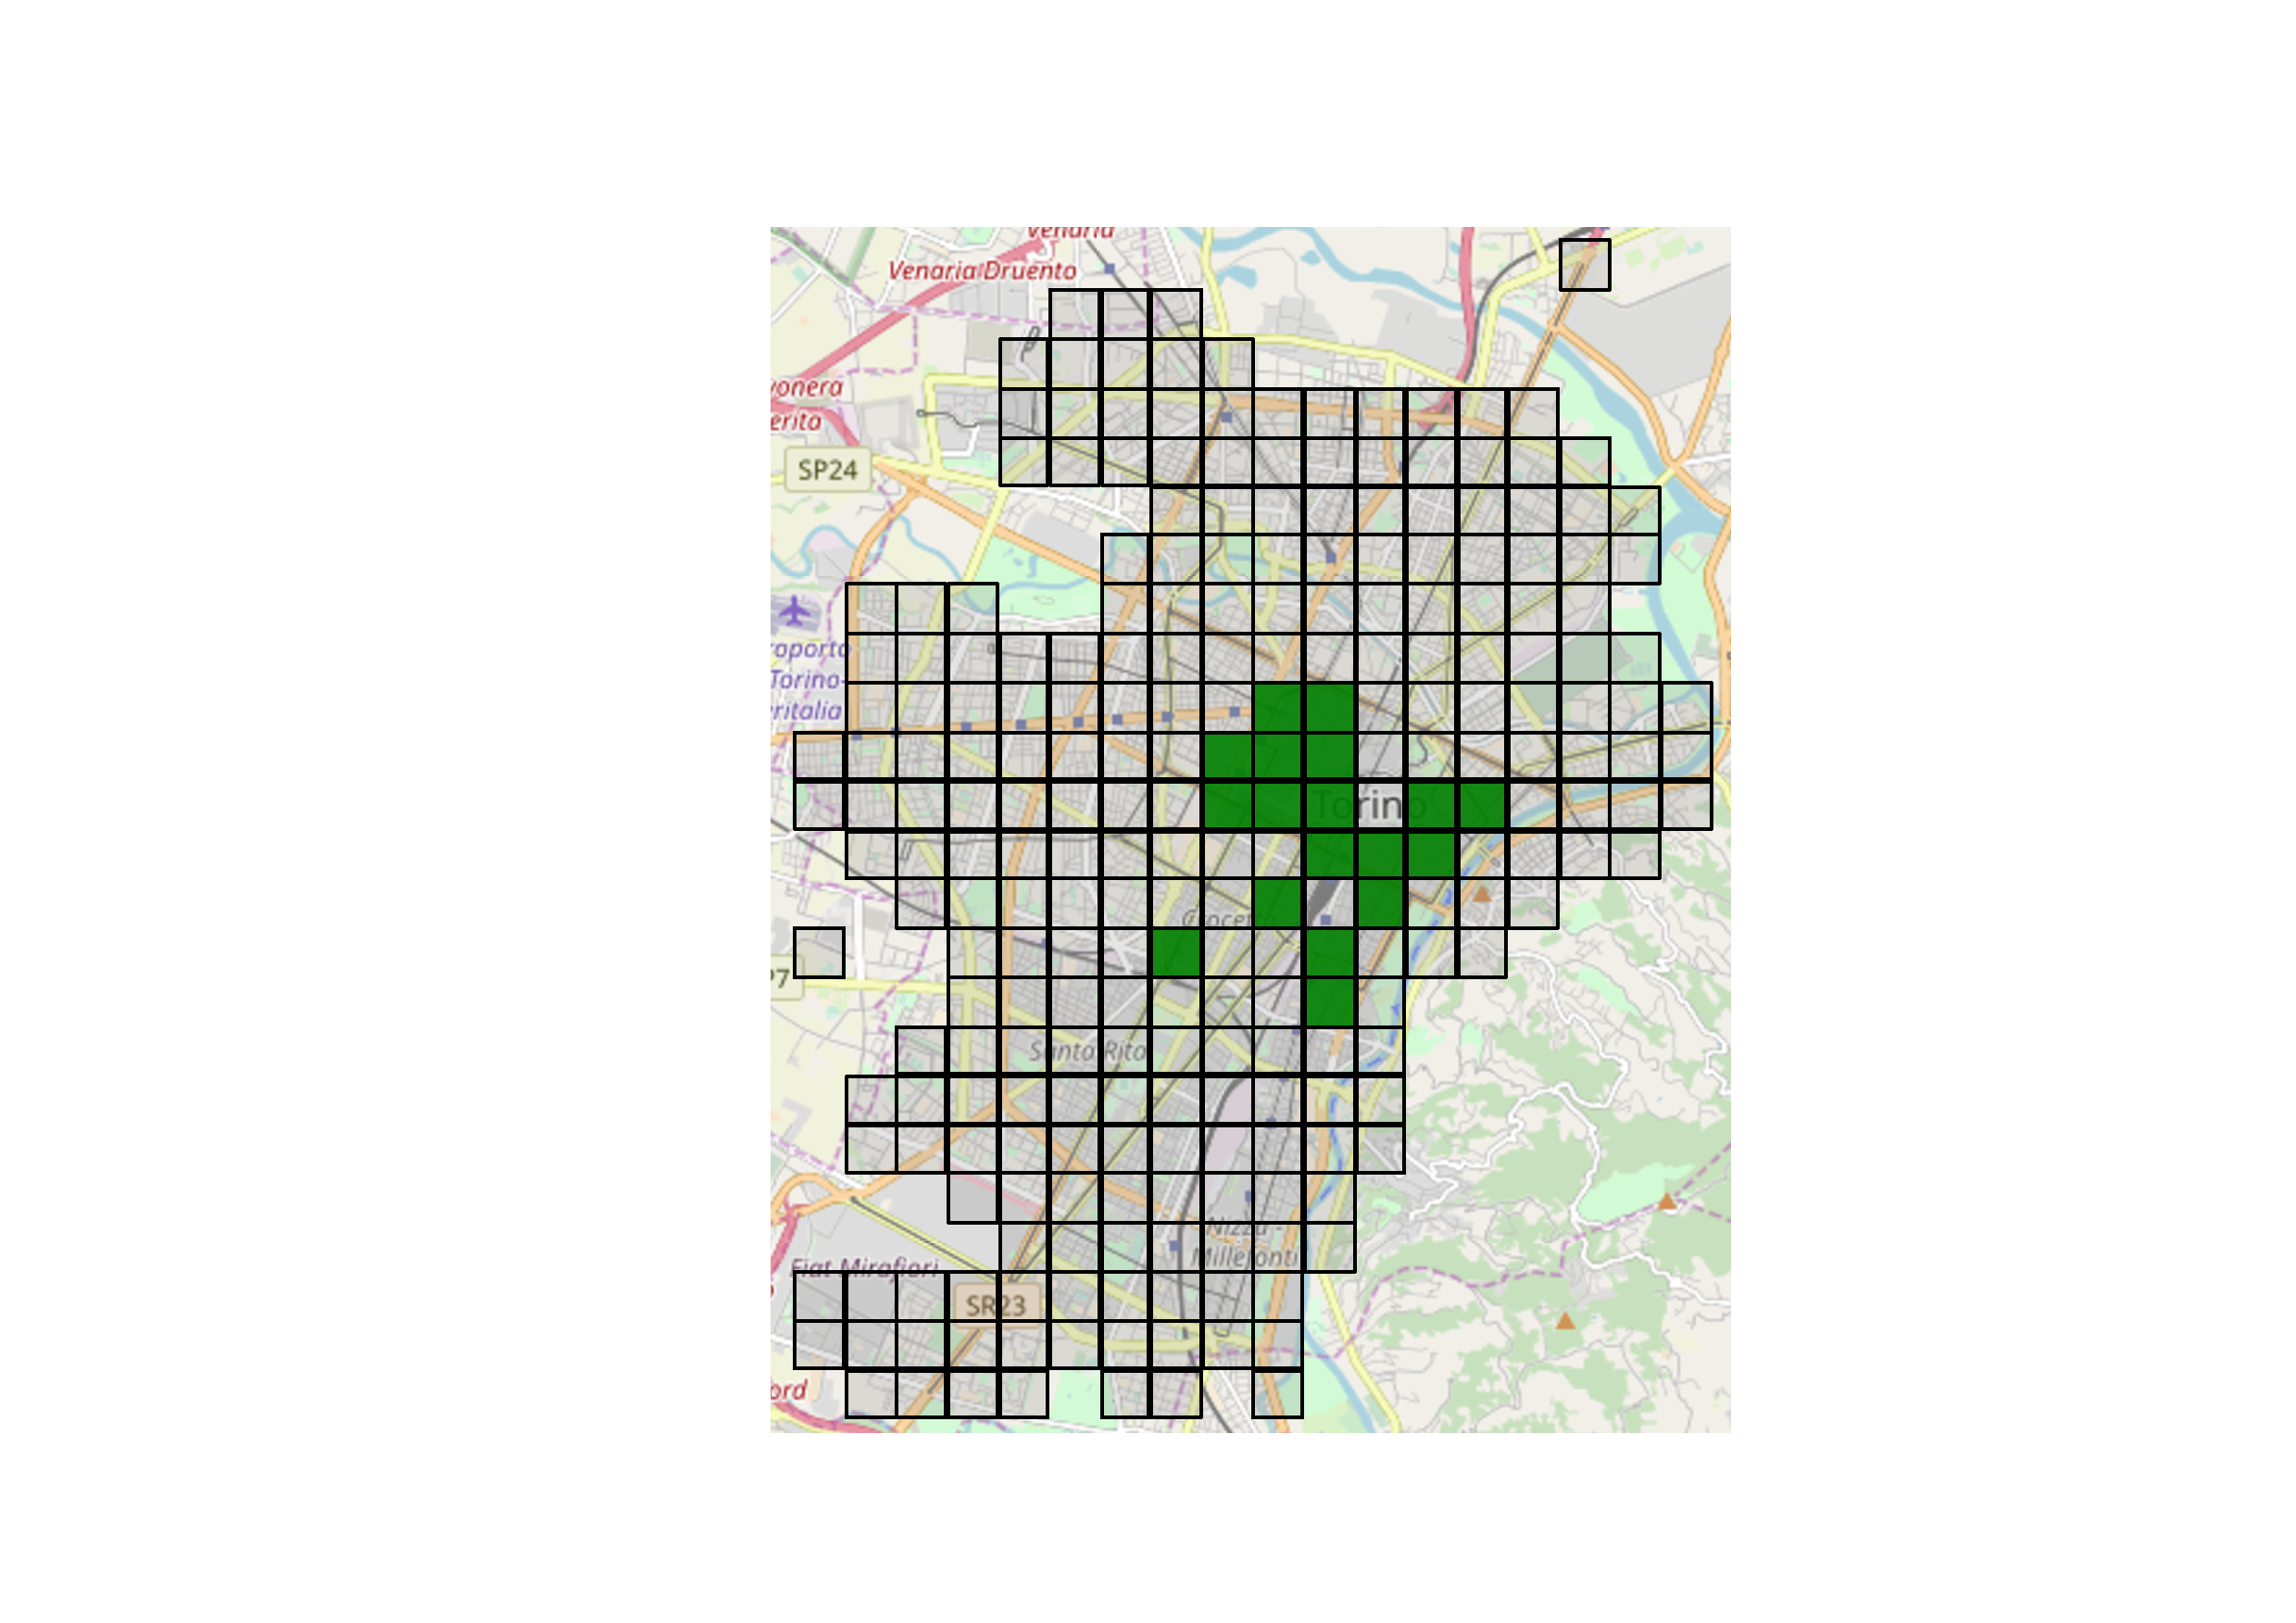
\includegraphics[width=0.3\columnwidth]{figures/NP_hybrid_18_Torino_placement.pdf}
        \label{fig:hm_max-parking_3}
    }
    \subfloat[][\textit{Local Search}.]
    {
        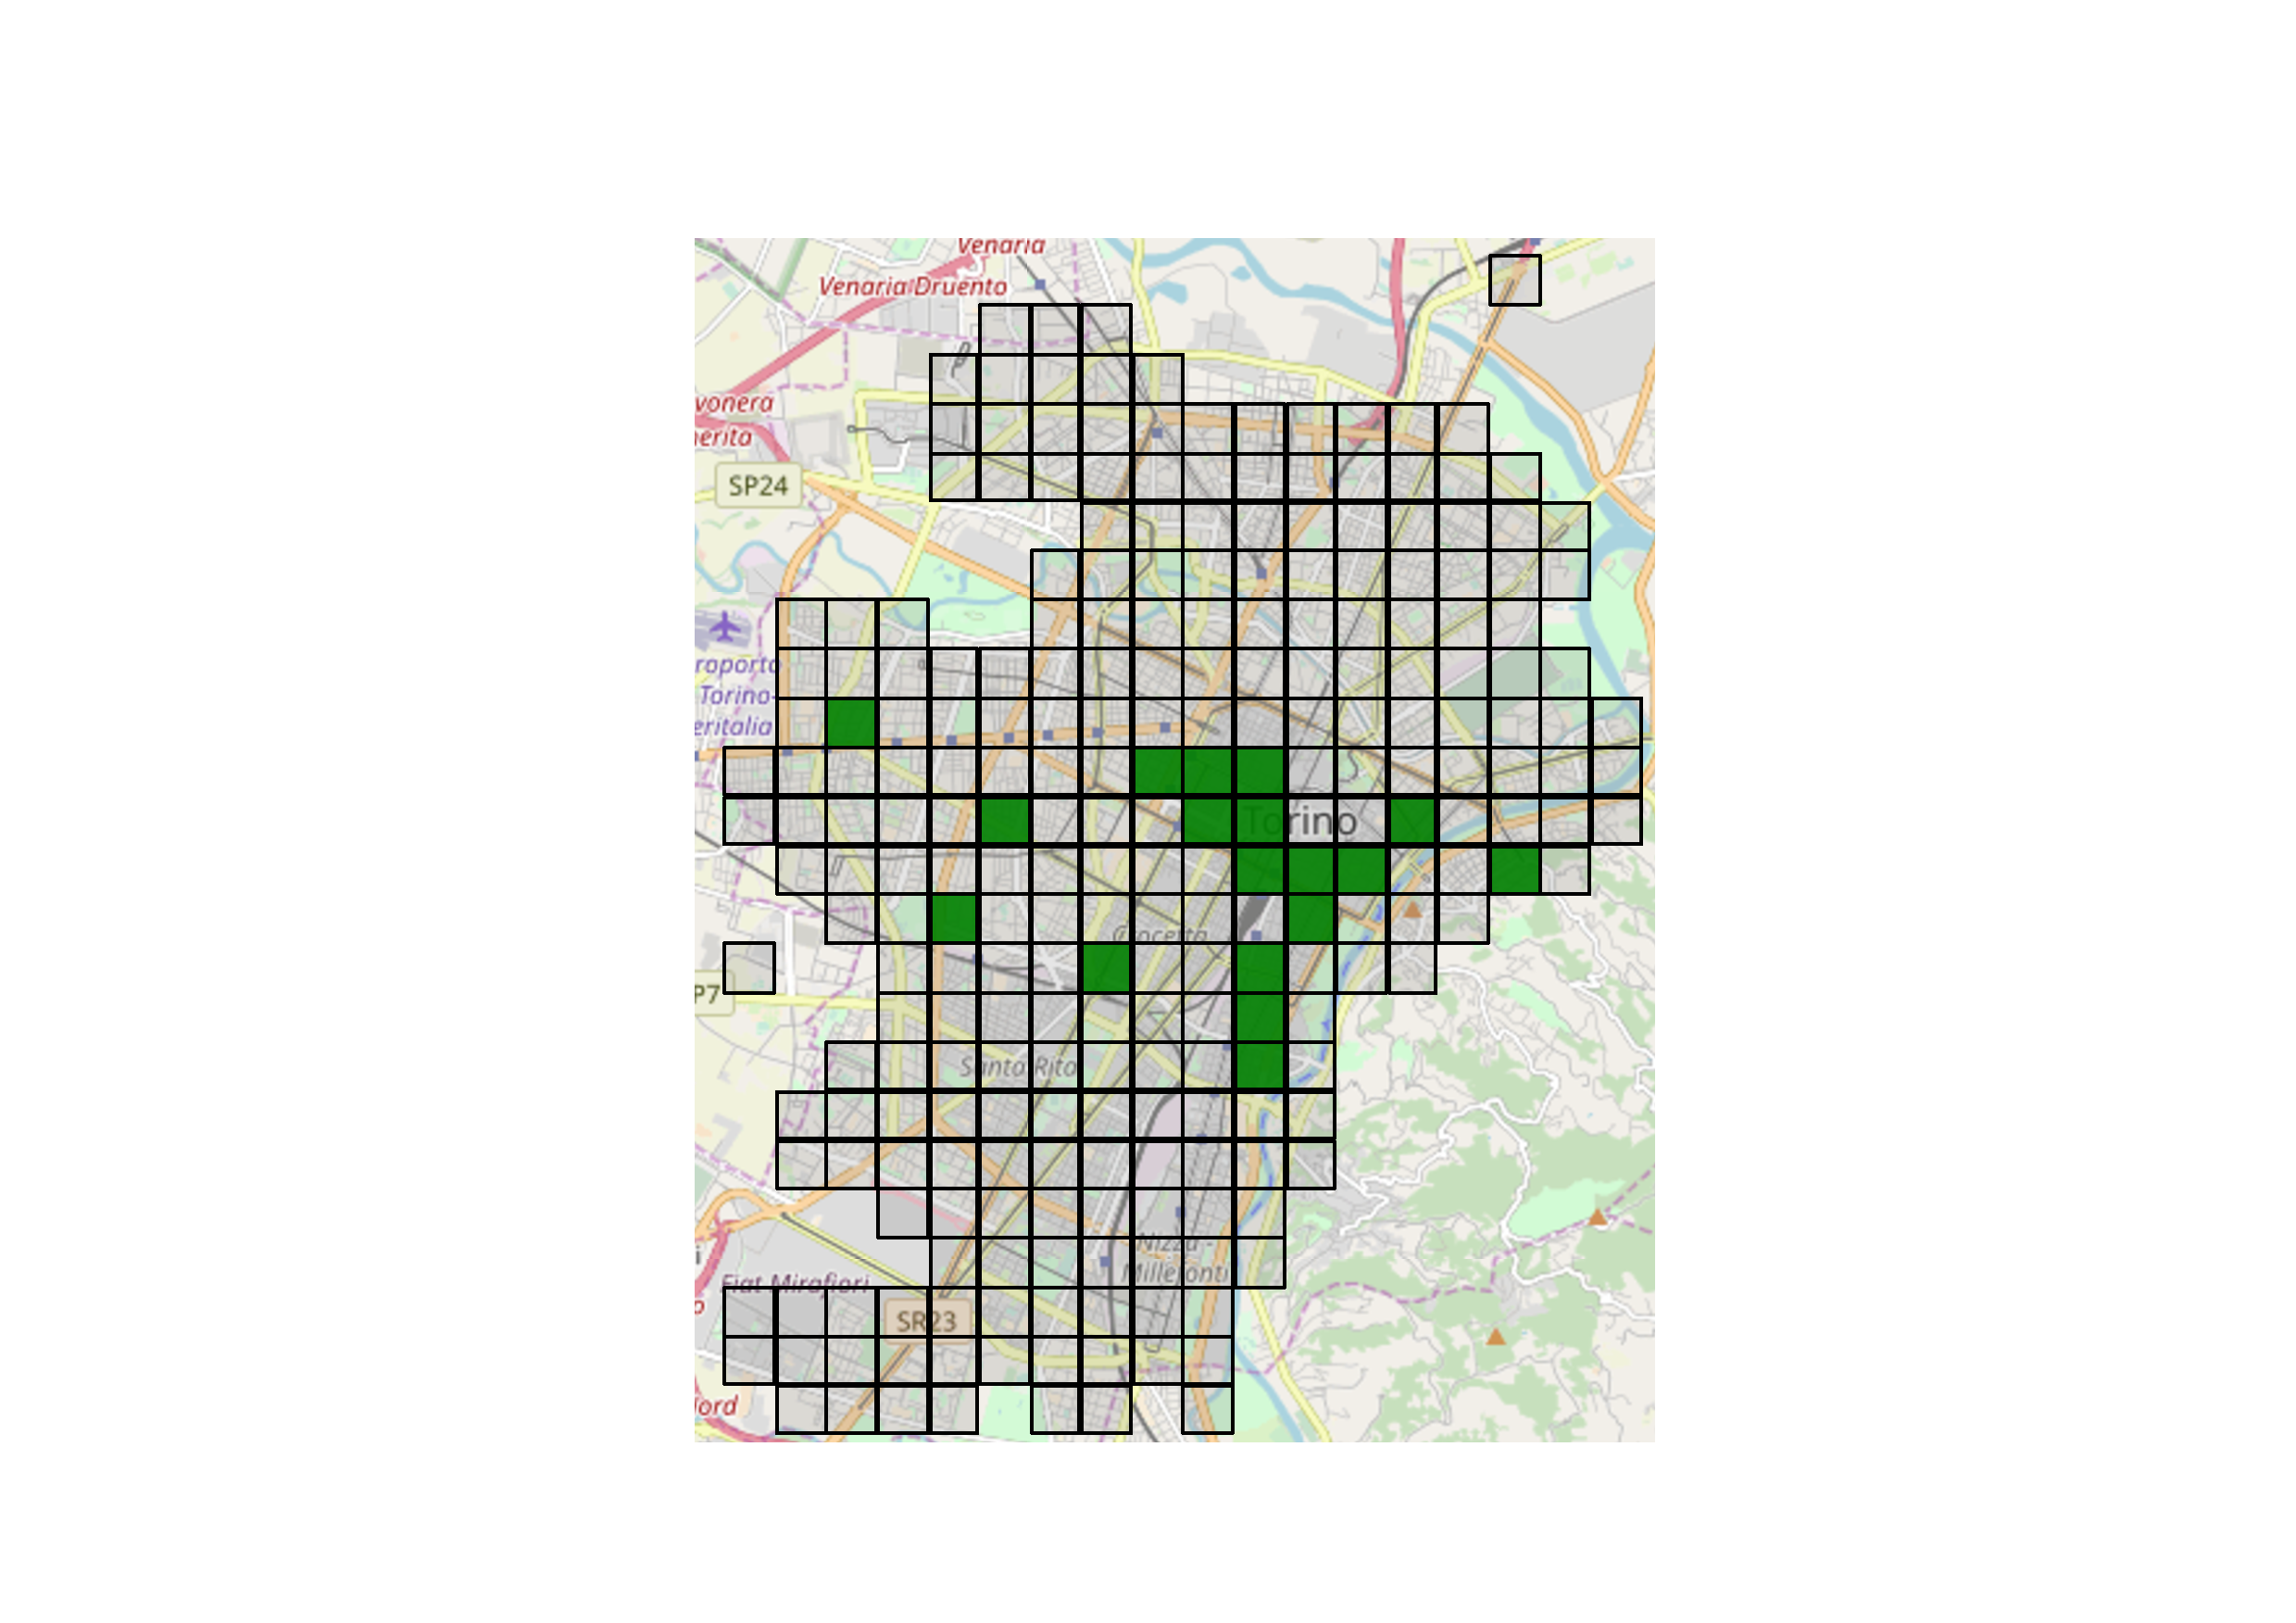
\includegraphics[width=0.3\columnwidth]{figures/LS_hybrid_18_Torino_placement.pdf}
        \label{fig:hm_local3}
    }
    \subfloat[][\textit{Genetic} algorithm.]
    {
        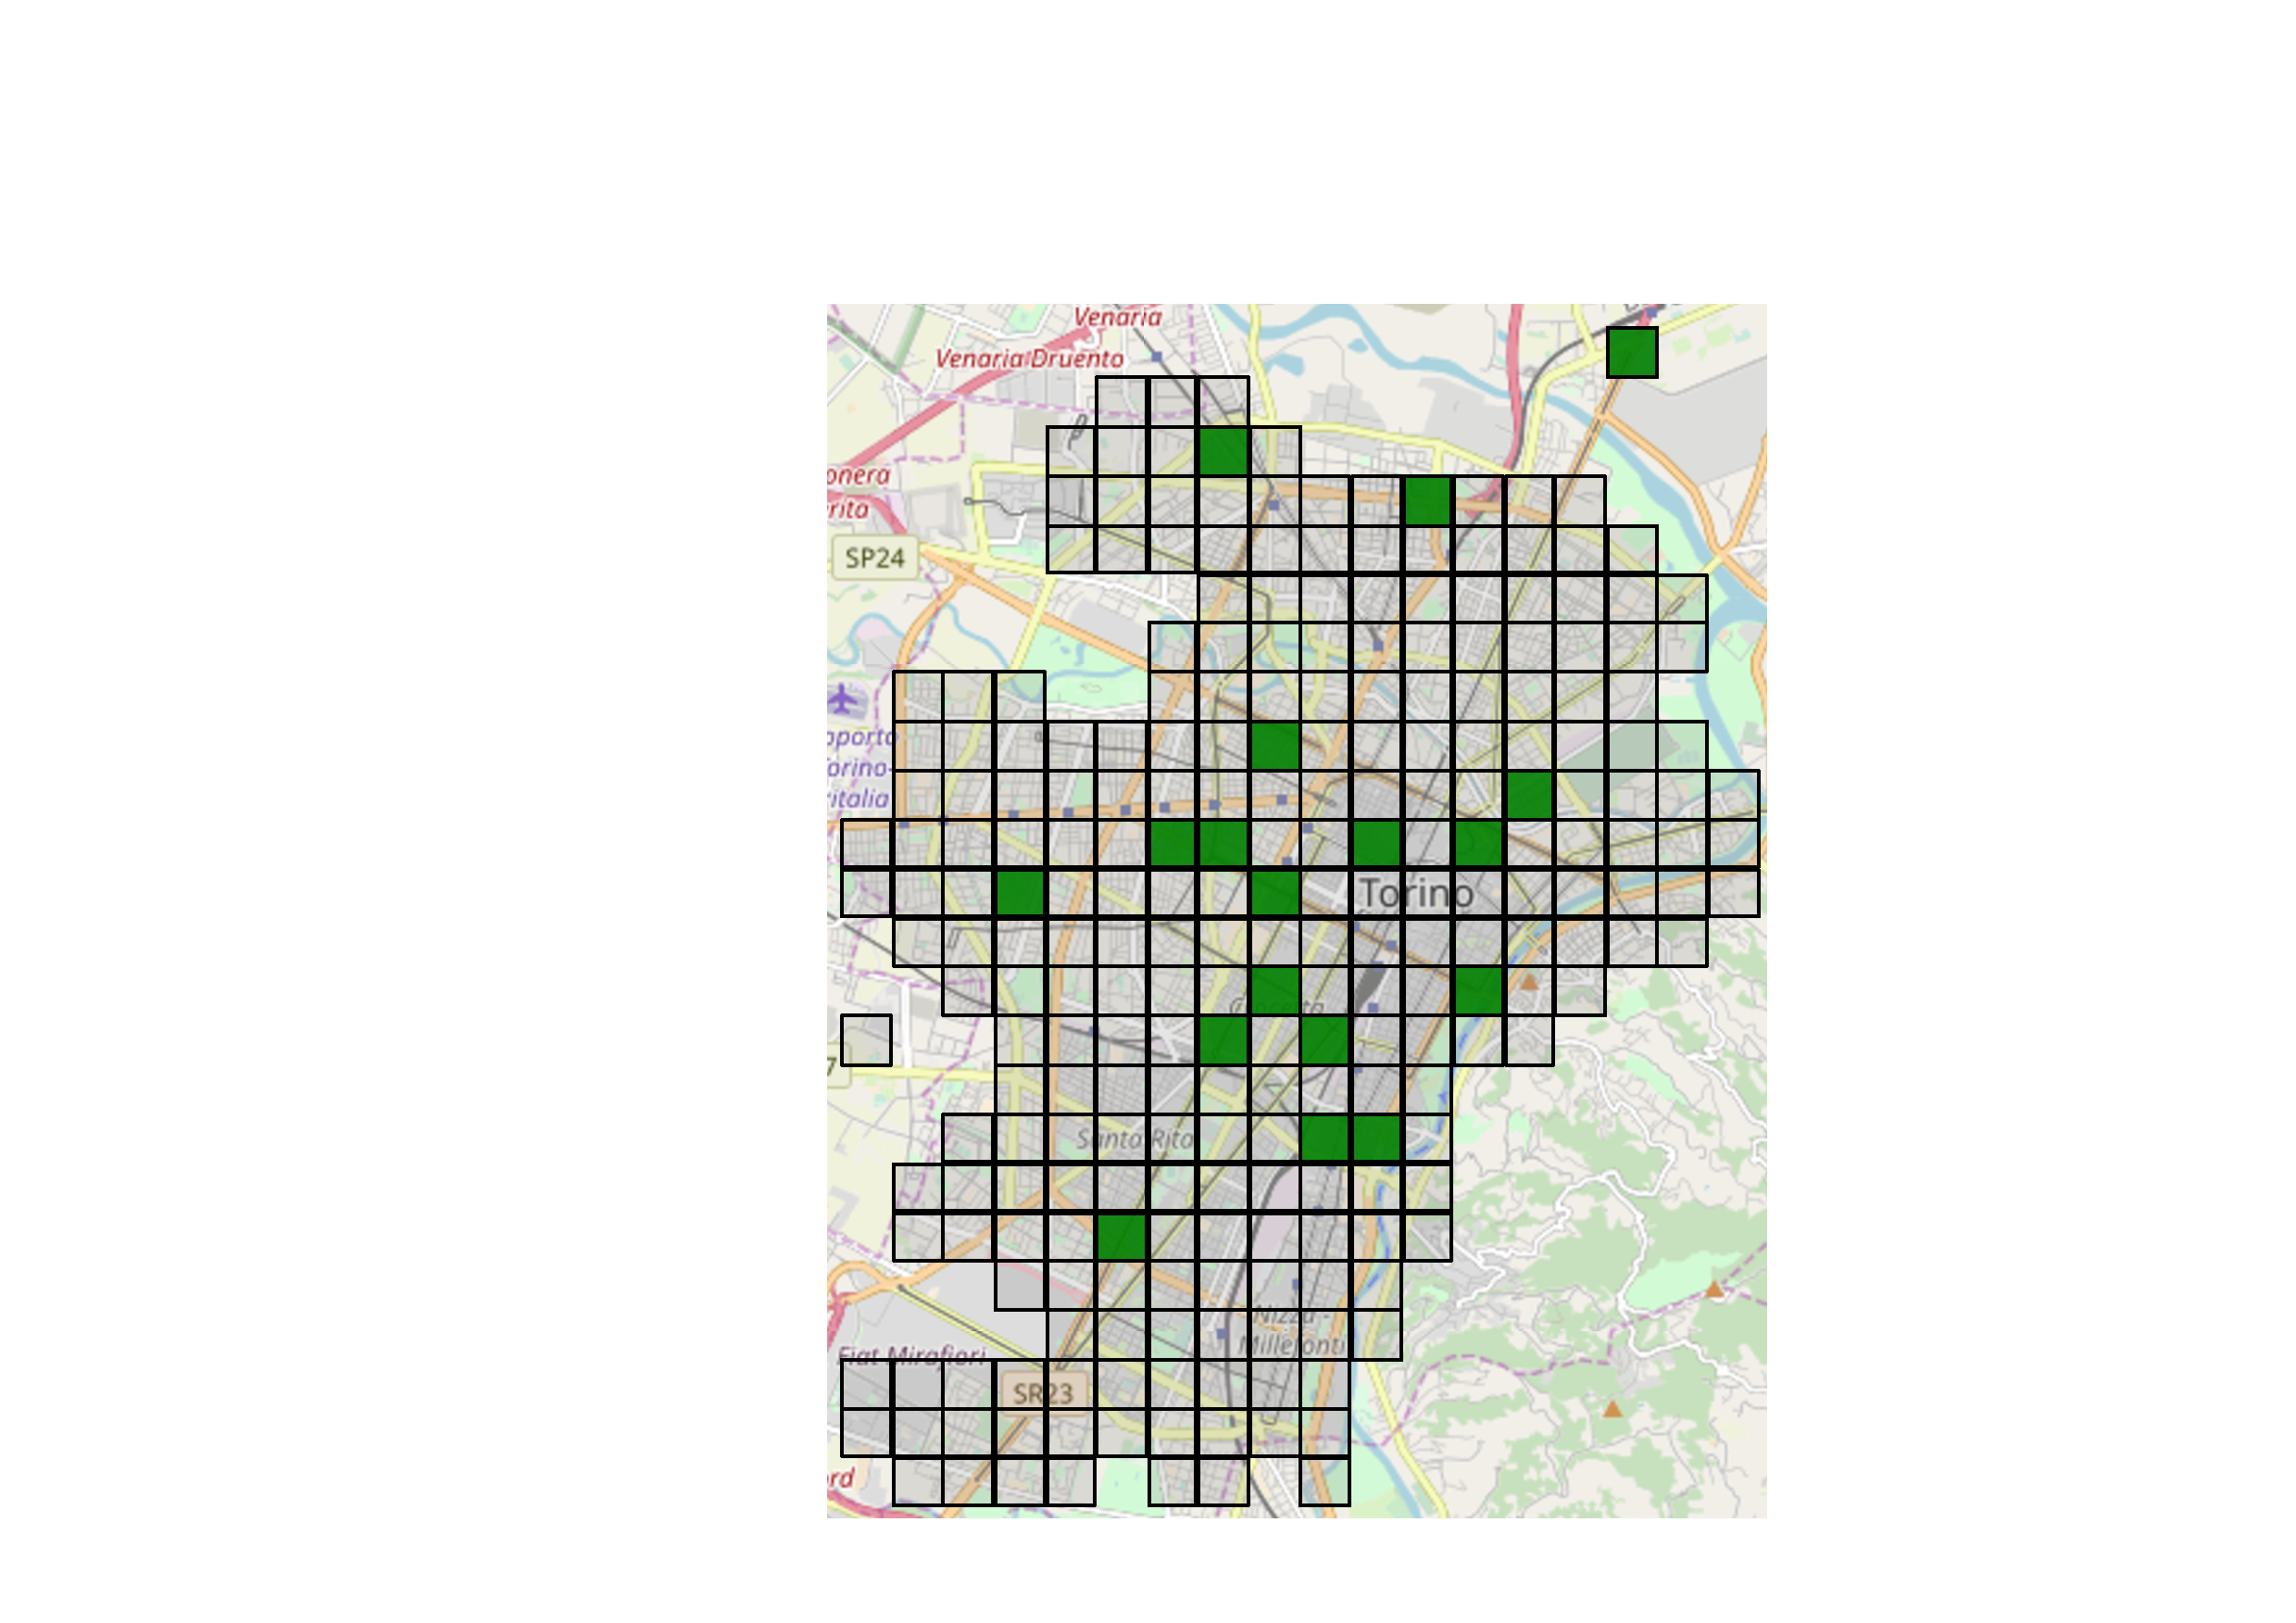
\includegraphics[width=0.3\columnwidth]{figures/GN_hybrid_18_Torino_placement.pdf}
        \label{fig:hm_genetico3}
    }
    \caption{Different placement of 18 zones (7\% of the total) for (a) Number of parkings per zone, (b) \textit{Local Search}  and (c) \textit{Genetic} solution. Darker areas have larger values.}
    \label{fig:maps}
\end{figure}

To give a feeling about the differences in the solutions found by different algorithms, Fig.~\ref{fig:maps} reports the solutions obtained with 7\% of the zones equipped with charging stations (i.e., $Z=18$ zones). %The upper right corner present in all figures refers to Turin airport (much further, in reality).  

\textit{Num parking} solution, Fig.~\ref{fig:hm_max-parking_3}, places most of the charging stations in downtown area and near the main train stations. 
\textit{Local Search}, Fig.~\ref{fig:hm_local3}, still has many zones in common with \textit{Num parking}, the solution it started from. It just spreads some charging station to cover also some remote zones.
The \textit{Genetic} algorithm, Fig.~\ref{fig:hm_genetico3}, shows very few zones in common with \textit{Num parking}. Charging stations are spread all over the city, still with more density in the city centre. %Moreover, the Turin airport is also a charging station zone, avoiding very long walks, a choice that the \textit{Local Search}, stuck in a local optimum, was not able to make. 
 


\subsection{Validation of optimised configurations}

\begin{figure}[t]
    \centering     %%% not \center
    \subfloat[][Percentage of infeasible trips. Y-Axis is logarithmic.]
    {
        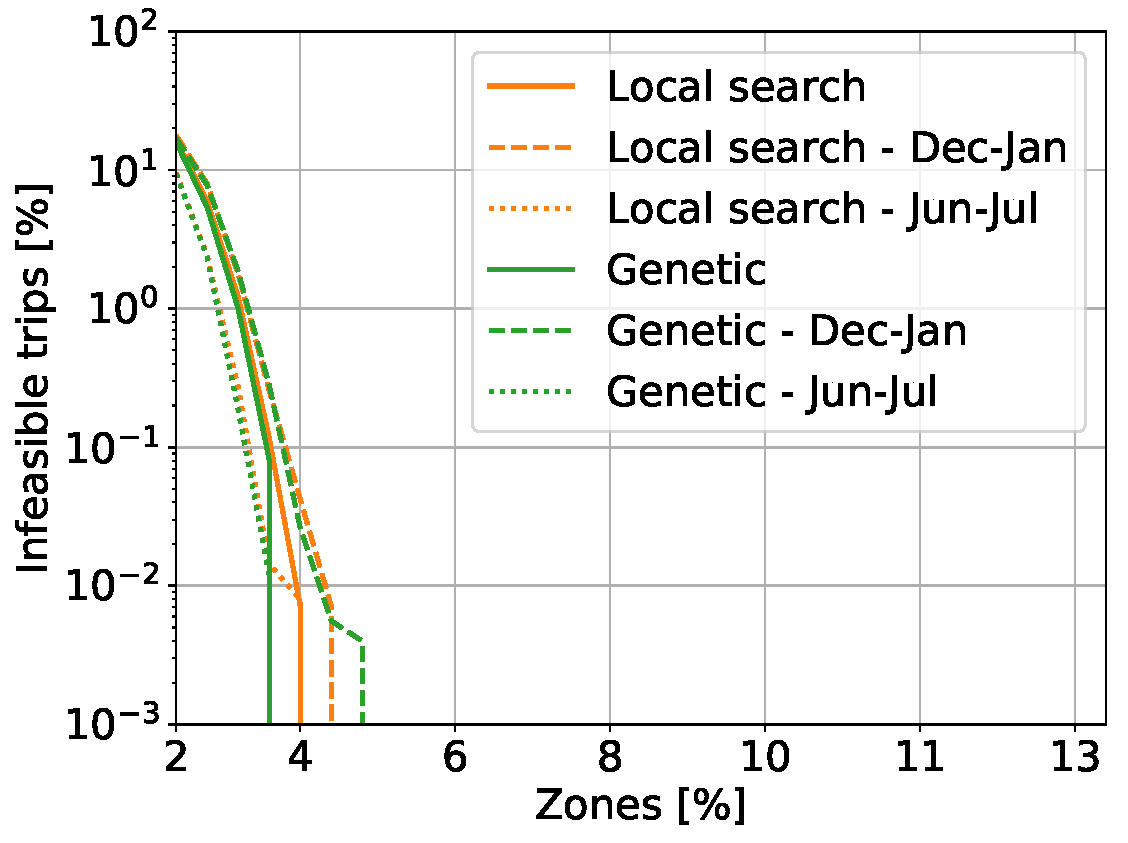
\includegraphics[width=0.45\columnwidth]{figures/Deaths_comparison.pdf}
        \label{fig:inf_validation}
    }
    \subfloat[][Walked distance, averaged over all trips.]
    {
        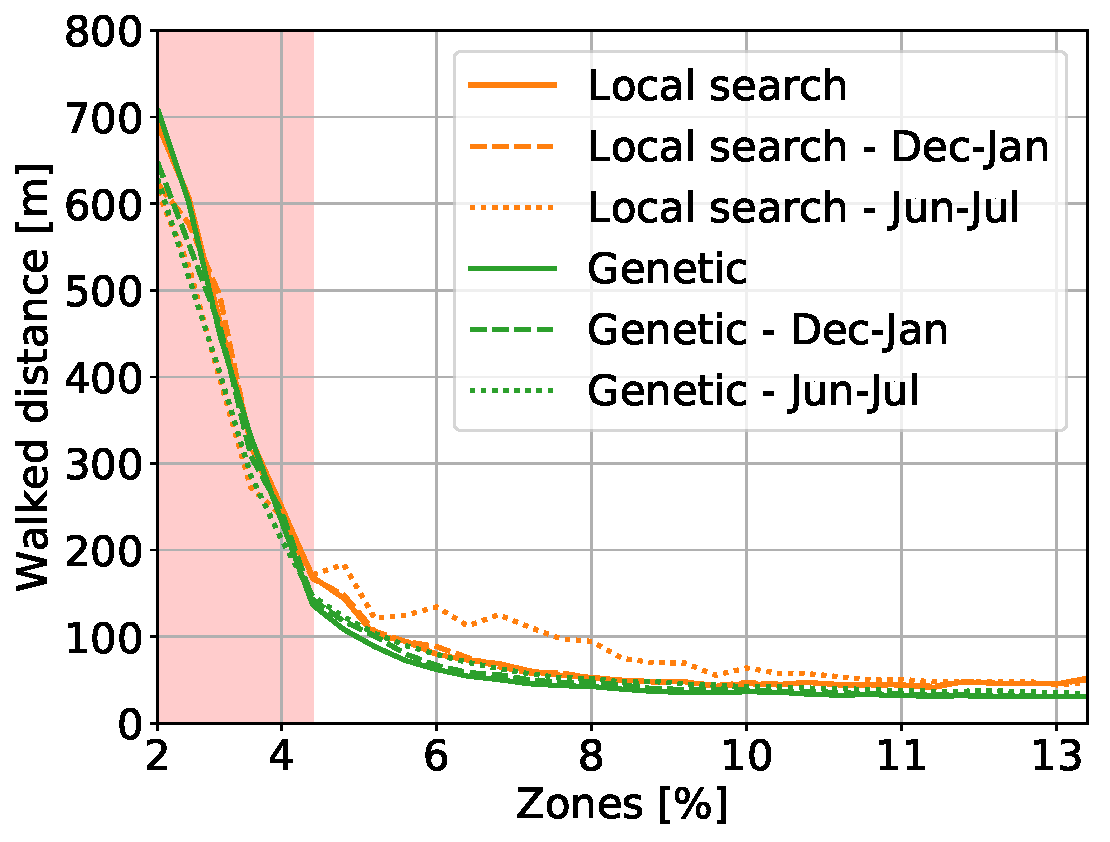
\includegraphics[width=0.45\columnwidth]{figures/TravelWithPenlaty_comparison.pdf}
        \label{fig:walked_validation}
    }

    \caption{Performance of the optimised configuration, tested on other 2 months long data-sets.}
    \label{fig:validation}
\end{figure}

\reviewed{The optimised solutions presented in the previous section are built through data-driven simulations. Hence they might over-fit the data of the specific considered period and not be robust to customers' habit changes. To validate our findings, we test the output placement configurations by using independent test traces, different from the one used to run the optimisation. 
% For this, we use the two different periods of two months: the latter selected in December 2017 and January 2018, collected in Turin again. For these two months we record 128\,780 rentals (3\% more trips than before). Instead the former takes in account June 2017 and July 2018 considering 101\,049 actual rentals. In this period the number of bookings 8\% lower due to beginning of European Summer. Those periods present different customers' habits, a hard challenge for the optimised configurations.
We rely on two traces collected in Turin in two different periods of the year: one in summer, from June to July 2017; the other in winter, from December 2017 to January 2018. We focus on these two periods since in summer and near Christmas holidays the users may exhibit different habits (e.g., customers may rent the cars to go to parks and swimming pools during summer). These anomalies may represent a challenge for the optimised configurations.
In the summer trace we record about  100\,000 rentals, while in the winter one 128\,000 rentals (respectively 8\% less and 3\% more with respect to the September/October trace). We compute the best station placement considering the September and October 2017 trace, and test system performance using the summer and winter traces.  

Fig.~\ref{fig:validation} compares results. We consider both \textit{Local Search} and \textit{Genetic} algorithms.
%\lv{diciamo negligibili come walked distance. Come infeasible trips cambiano, piu delle figure mostrate sopra sugli infeasible trips. Ma trattandosi di poche morti, anche solo la parte randomica va a influire abbastanza}
%As we can see, both figures have curves whit similar trends
% Differences are negligible, showing that optimisation results are robust. For example, for 13\% of zones and considering \textit{Genetic} algorithm, the walked distance on the test is just 2\,m above the one in the optimised trace. 
In almost all cases, differences are negligible, showing that the solution is robust. For example, for 13\% of zones and considering \textit{Genetic} algorithm, the walked distance on the tests are just 2\,m above those in the trace used for optimisation. Notice how in June and July the \textit{Local Search} behaves worse than other cases: this is possibly due to the different mobility patterns in summer, while the Local Search solution could still be too related to the number of parkings in September-October. On the other hand, the solution found by the global genetic algorithm is robust.
%In any case this behaviour is noticeable considering few charging stations: considering more than 13\% of zones the placements have the same performances.
}
%In the test set, the number of infeasible trips goes to 0 needing up to 3 additional zones for both genetic and local search. Regarding the walked distance, for 13\% of zones, the genetic algorithm walked distance on the test is just 2\,m above the one optimized on the original dataset. 
%Concluding, our placement solutions do not overfit the trace used for the designing and seem robust with respect to the change of habits.
